\section{Advanced analyses}

\subsection{Climate analysis}
For every city we fit temperature on a linear trend, two annual harmonics, and two diurnal harmonics of the
snapshot hour. The record covers only about 2.4 years, so these slopes describe short-term variation, not
climate change. Without the hour terms, 79\,\% of cities appear to cool, at a median of $-1.79$\,\textdegree C/yr.
With them the median slope falls to $-0.51$\,\textdegree C/yr (Figure~\ref{fig:climtrend}). The diurnal effect
captured by the hour terms is large: about 8\,\textdegree C peak-to-peak in the median city.
Seasonality is structured by latitude. The two hemispheres run in opposite phase
(Figure~\ref{fig:latband}), and the annual range grows strongly with $|$latitude$|$ ($r=0.84$). Continental
capitals such as Ulaanbaatar, Astana and Bishkek have the widest swings (30--42\,\textdegree C) (Figure~\ref{fig:amp}).

\begin{figure}[H]\centering
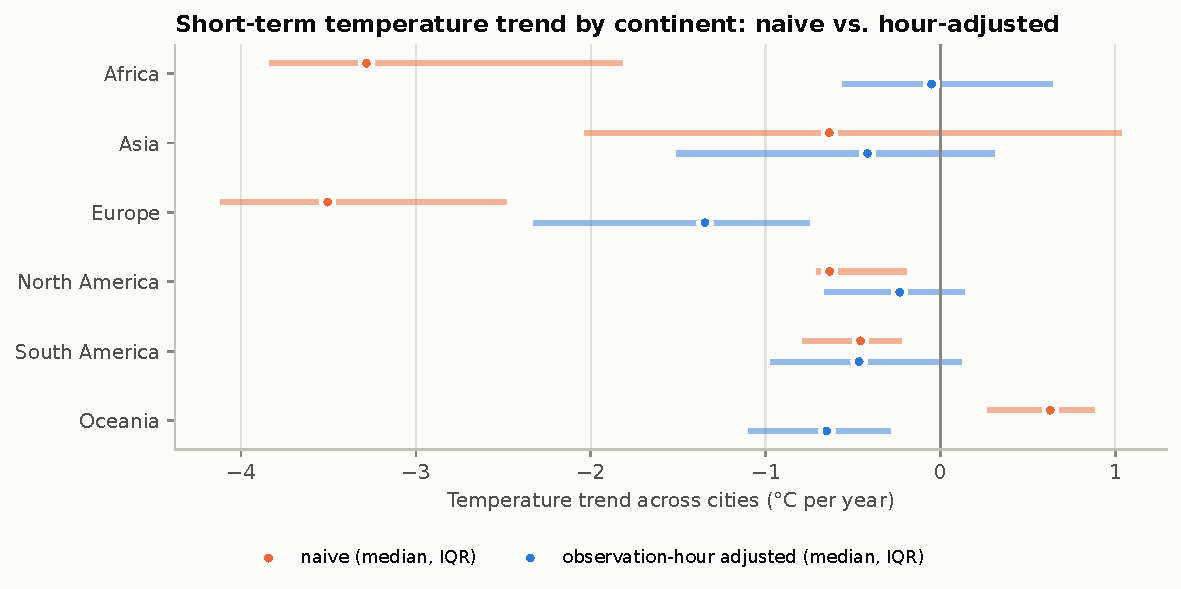
\includegraphics[width=0.85\linewidth]{analyses/climate_trend_by_continent}
\caption{Per-city temperature trends by continent, naive and observation-hour adjusted.}\label{fig:climtrend}
\end{figure}
\begin{figure}[H]\centering
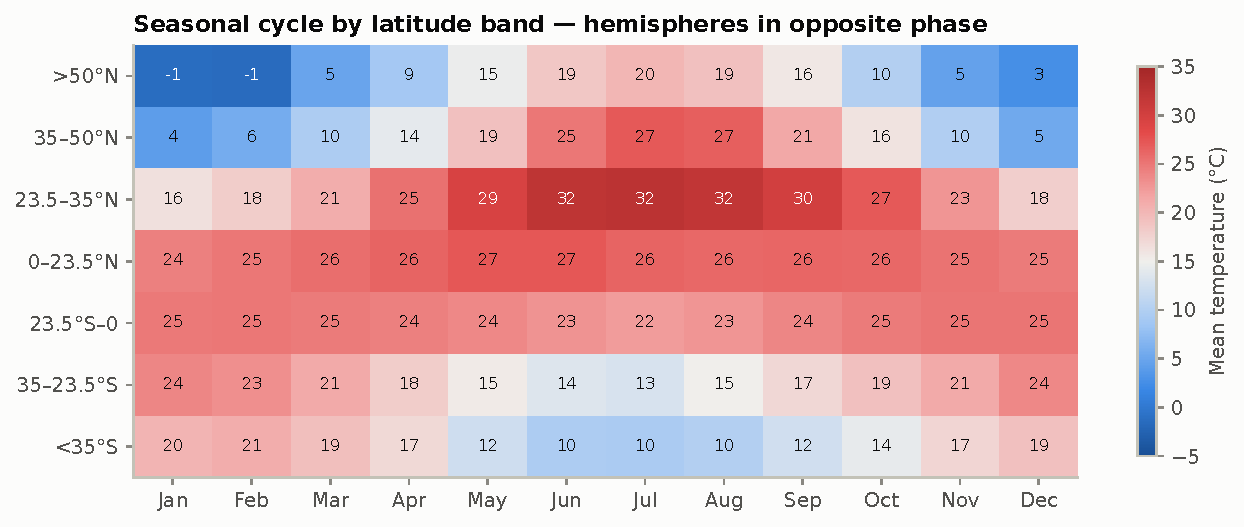
\includegraphics[width=0.9\linewidth]{analyses/climate_latitude_band_seasonality}
\caption{Mean temperature by latitude band and calendar month.}\label{fig:latband}
\end{figure}
\begin{figure}[H]\centering
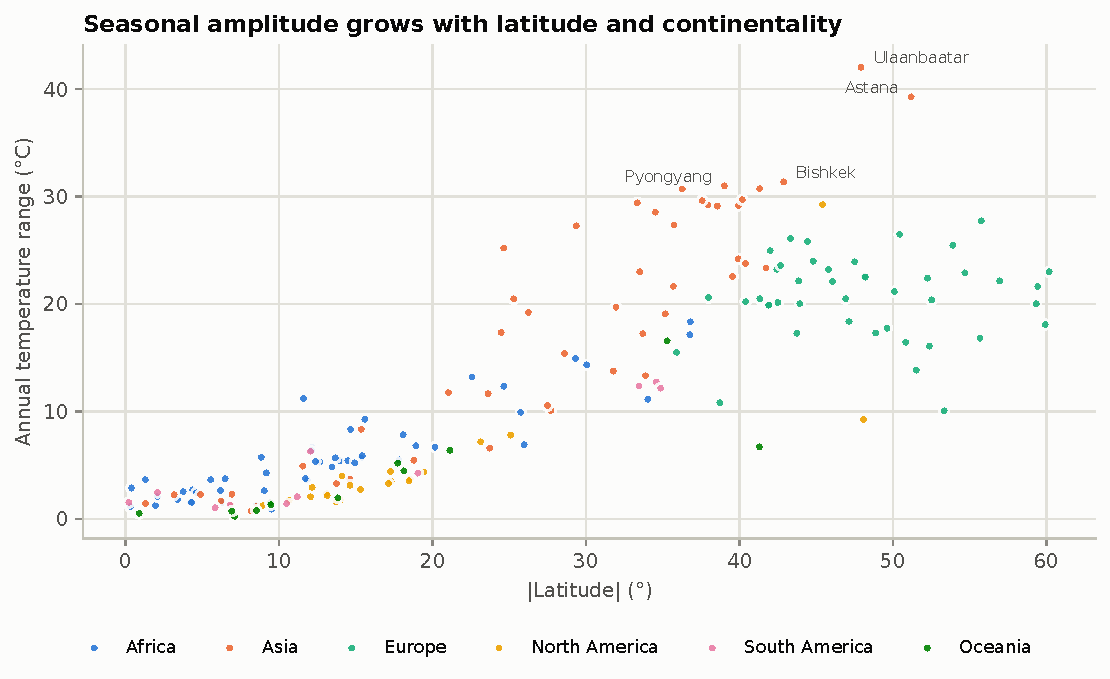
\includegraphics[width=0.75\linewidth]{analyses/climate_amplitude_vs_latitude}
\caption{Annual temperature range against $|$latitude$|$.}\label{fig:amp}
\end{figure}

\subsection{Environmental impact: air quality and weather}
Pooled correlations mix geography with weather: humid tropical capitals are cleaner than dry, dense ones.
To isolate the weather effect we also compute \emph{within-city} correlations, after removing each city's mean
(Figure~\ref{fig:aqcorr}).
\begin{itemize}
  \item \textbf{Ozone} is photochemical. It rises with temperature ($\rho=0.31$) and UV ($\rho=0.32$) and
        falls with humidity.
  \item \textbf{NO$_2$} and \textbf{SO$_2$} fall with wind (dispersion) and rise with pressure (stagnant
        anticyclones).
  \item \textbf{PM2.5} falls with wind, precipitation and cloud (wash-out and mixing). Within a city these
        effects are weak ($|\rho|\le0.13$), so particulate levels are driven mostly by local emissions.
\end{itemize}
A LightGBM model of $\log$\,PM2.5 reaches test $R^2\approx0.51$. Location (longitude and latitude) dominates
its permutation importance, calendar month barely matters, and UV, temperature and humidity are the main weather
drivers (Figure~\ref{fig:pmdrivers}). The median
PM2.5 of 41\,\% of capitals exceeds the WHO 24-hour guideline of 15\,µg/m³. Asia carries the heaviest burden.

\begin{figure}[H]\centering
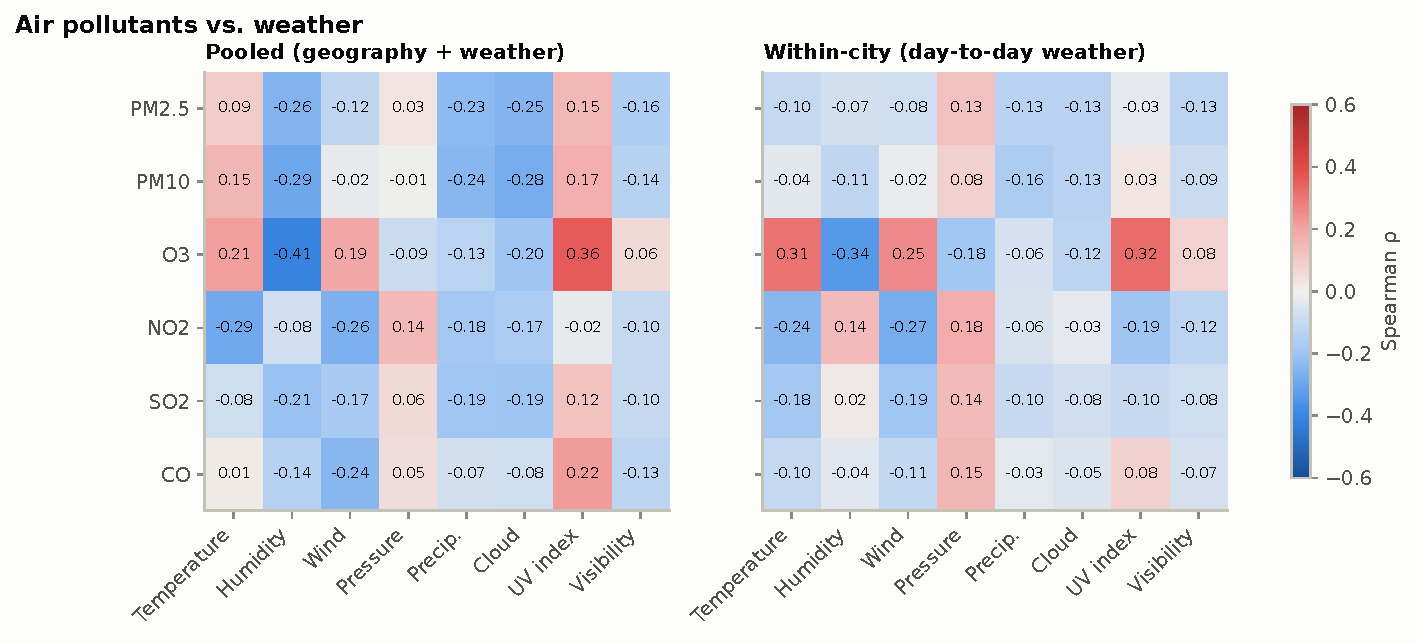
\includegraphics[width=\linewidth]{analyses/airquality_weather_correlation}
\caption{Air pollutants against weather: pooled (left) and within-city (right) Spearman correlations.}\label{fig:aqcorr}
\end{figure}
\begin{figure}[H]\centering
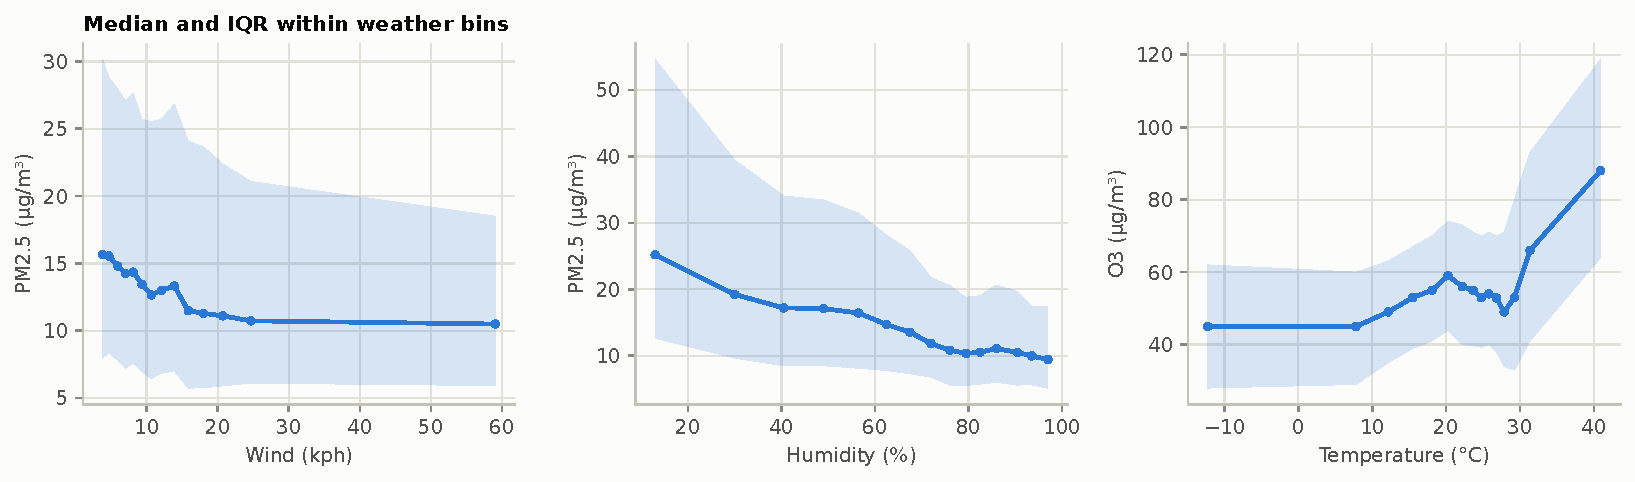
\includegraphics[width=\linewidth]{analyses/airquality_response_curves}
\caption{Pollutant response within weather bins (median and IQR).}
\end{figure}
\begin{figure}[H]\centering
\begin{subfigure}{0.49\linewidth}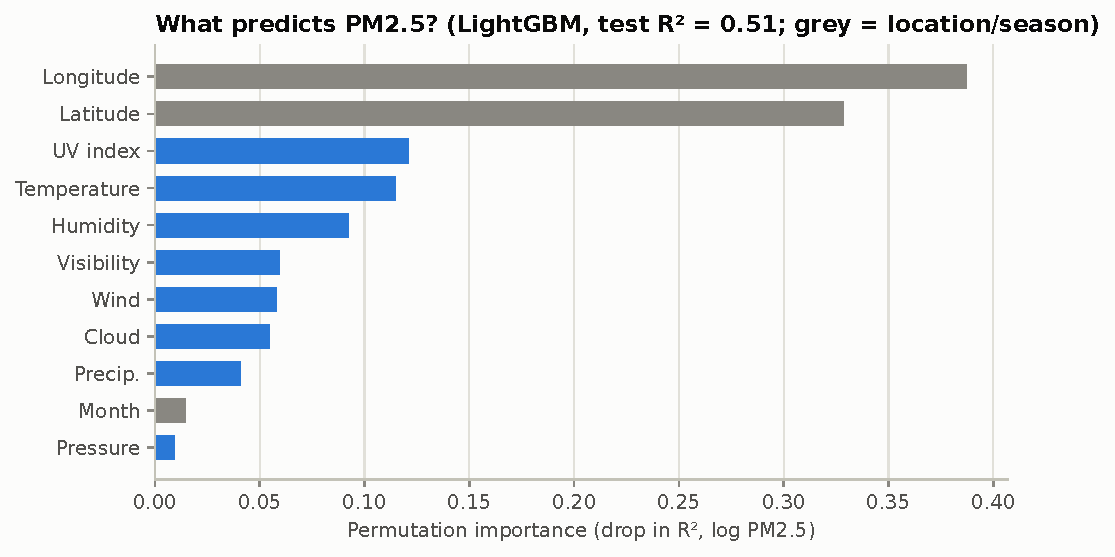
\includegraphics[width=\linewidth]{analyses/airquality_pm25_drivers}\caption{Drivers of PM2.5}\label{fig:pmdrivers}\end{subfigure}
\begin{subfigure}{0.49\linewidth}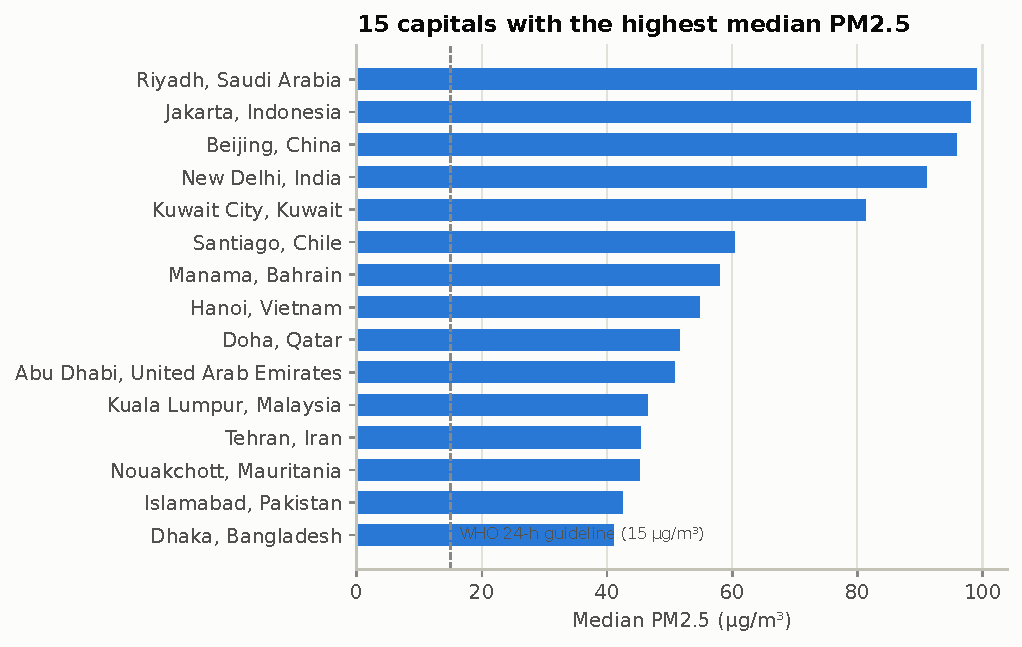
\includegraphics[width=\linewidth]{analyses/airquality_top_pm25}\caption{Most polluted capitals}\end{subfigure}
\caption{Air-quality drivers and hotspots.}
\end{figure}
\begin{figure}[H]\centering
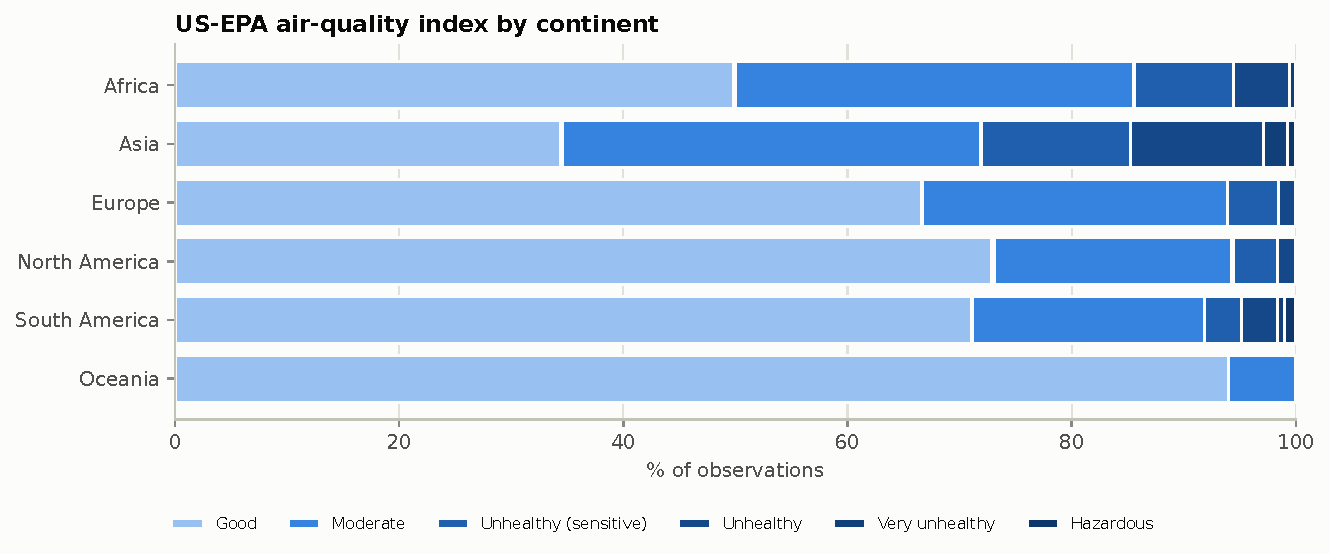
\includegraphics[width=0.9\linewidth]{analyses/airquality_epa_by_continent}
\caption{US-EPA air-quality index categories by continent.}
\end{figure}

\subsection{Feature importance}
Feature importance for the LightGBM next-day model is assessed four ways: split \textbf{gain},
\textbf{permutation} (increase in test RMSE), \textbf{mean $|$SHAP$|$} (TreeExplainer) and \textbf{mutual
information}. All four agree that persistence dominates: current temperature first, then its 3-, 7- and 14-day
rolling means and the feels-like temperature (Table~\ref{tab:feature_importance}). Gain and SHAP rankings
correlate at $\rho=0.73$, and permutation and SHAP at $\rho=0.83$. Mutual information also rewards redundant
features, such as raw lags, that the trees do not need. Past the persistence block, the secondary signals are
humidity, pressure and its daily change, latitude, UV, and the diurnal snapshot-hour terms
(Figure~\ref{fig:fi2}).

\tbl{feature_importance.tex}
\begin{figure}[H]\centering
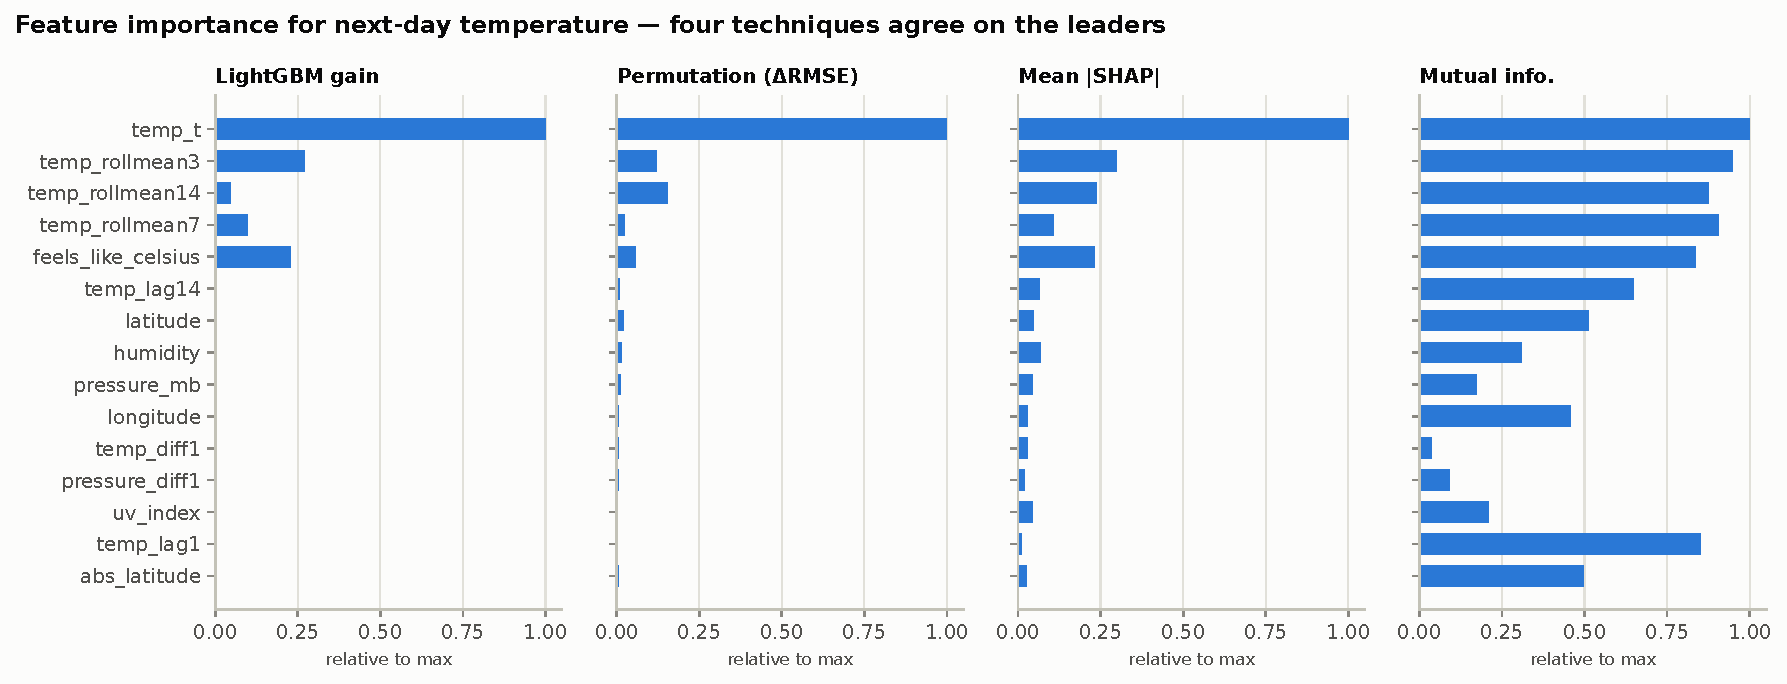
\includegraphics[width=\linewidth]{analyses/feature_importance_comparison}
\caption{Top-15 features under four importance techniques, each scaled to its maximum.}
\end{figure}
\begin{figure}[H]\centering
\begin{subfigure}{0.49\linewidth}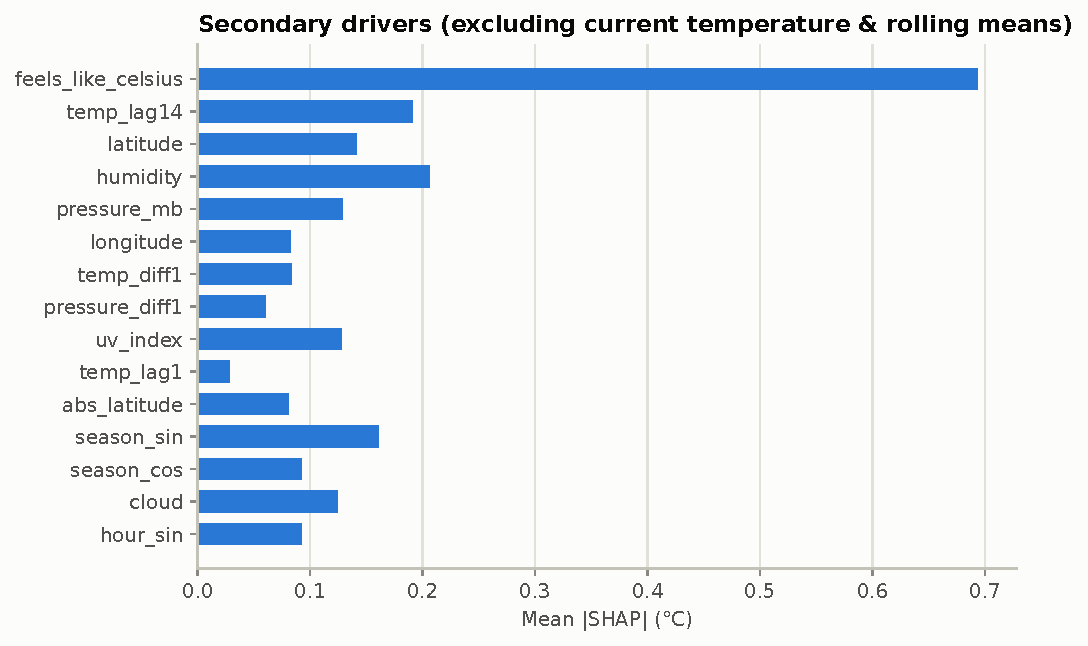
\includegraphics[width=\linewidth]{analyses/feature_importance_secondary}\caption{Secondary drivers}\label{fig:fi2}\end{subfigure}
\begin{subfigure}{0.49\linewidth}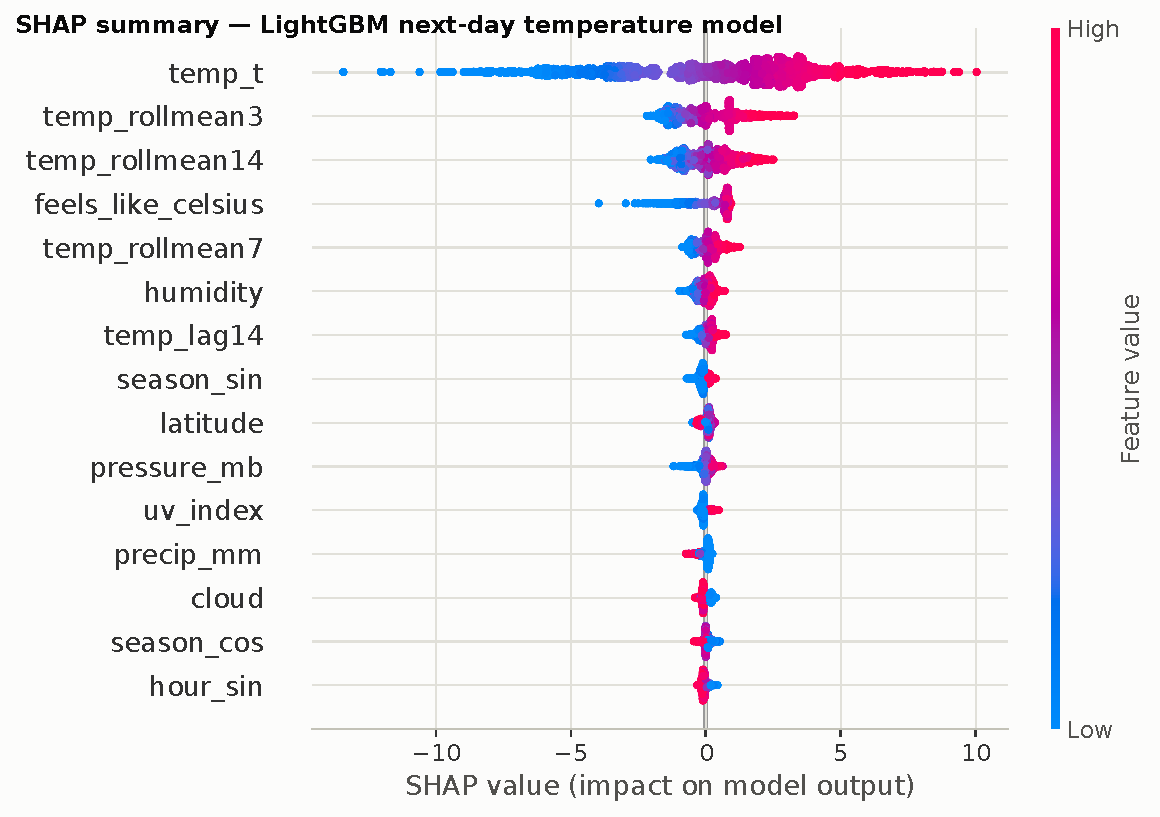
\includegraphics[width=\linewidth]{analyses/feature_importance_shap_summary}\caption{SHAP summary}\end{subfigure}
\caption{Feature importance beyond persistence, and a SHAP beeswarm.}
\end{figure}

\subsection{Spatial analysis}
Every variable is clustered in space. Moran's $I$ with 8-nearest-neighbour great-circle weights and 999
permutations gives $p=0.001$ for all four variables (Figure~\ref{fig:spatial}): temperature $I=0.68$,
humidity $0.71$, precipitation $0.54$ and PM2.5 $0.31$. PM2.5 is the least spatially structured because it
depends on local emissions. Temperature declines away from the equator, faster in the Northern Hemisphere,
where most high-latitude capitals lie (Figure~\ref{fig:latprof}). Interactive maps are produced in
\texttt{reports/maps/}: a Folium map of all capitals with pop-ups, and Plotly maps.

\begin{figure}[H]\centering
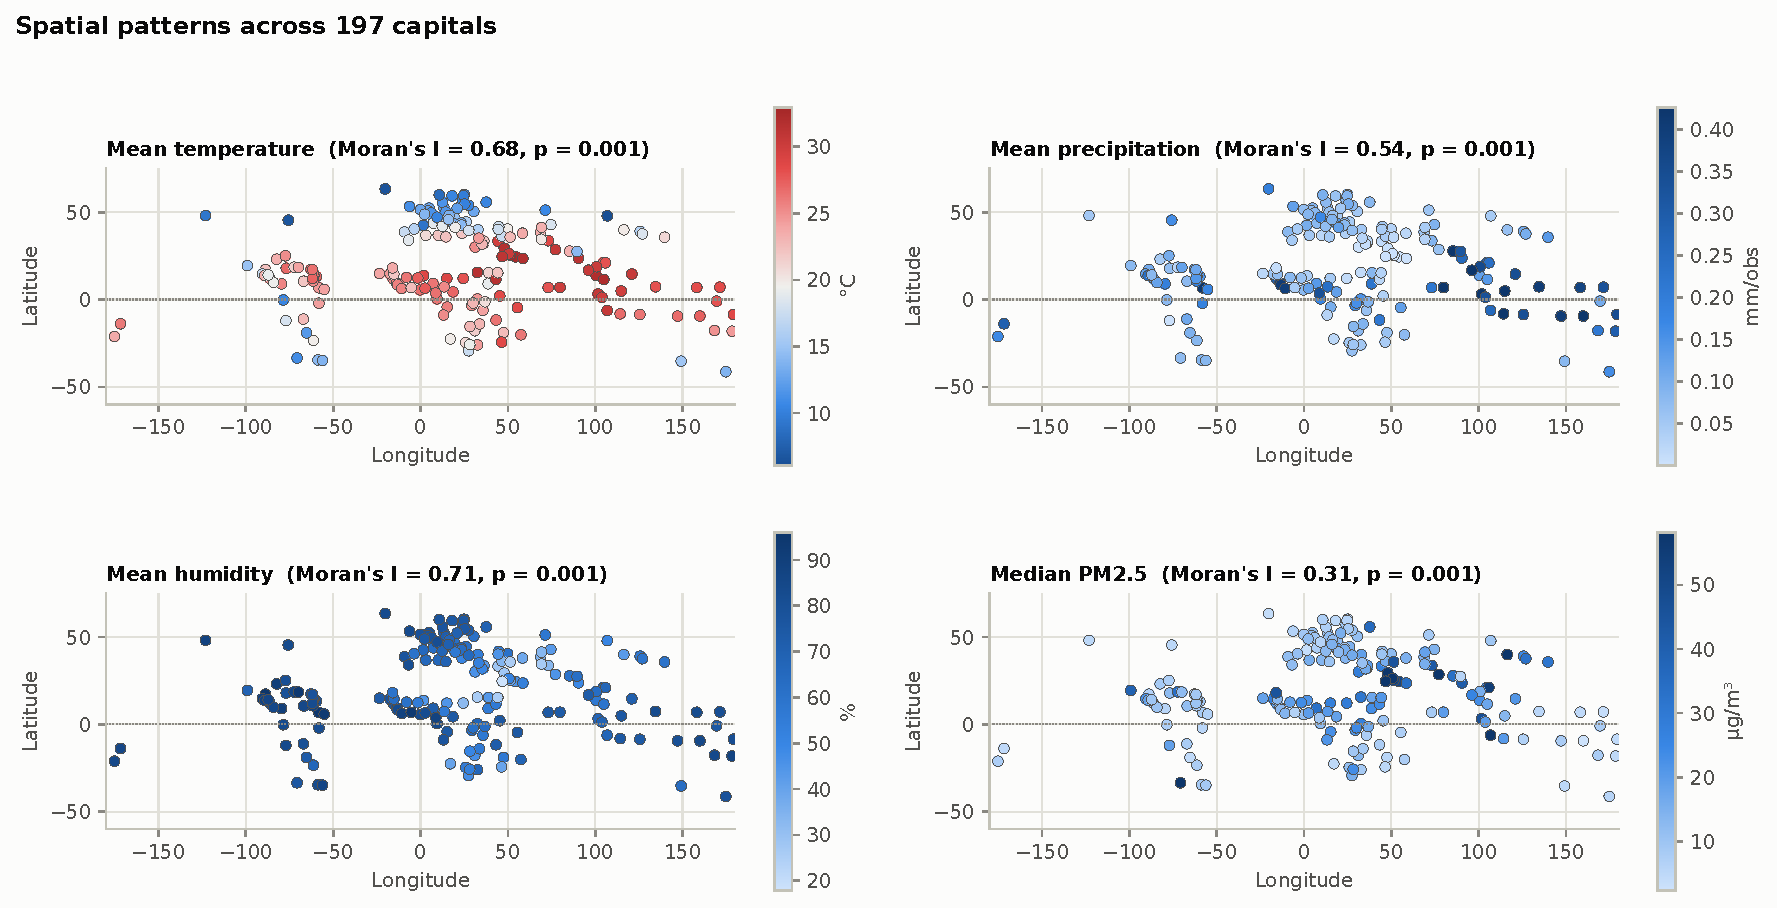
\includegraphics[width=\linewidth]{analyses/spatial_maps}
\caption{Spatial distribution of climate and air quality, with Moran's $I$.}\label{fig:spatial}
\end{figure}
\begin{figure}[H]\centering
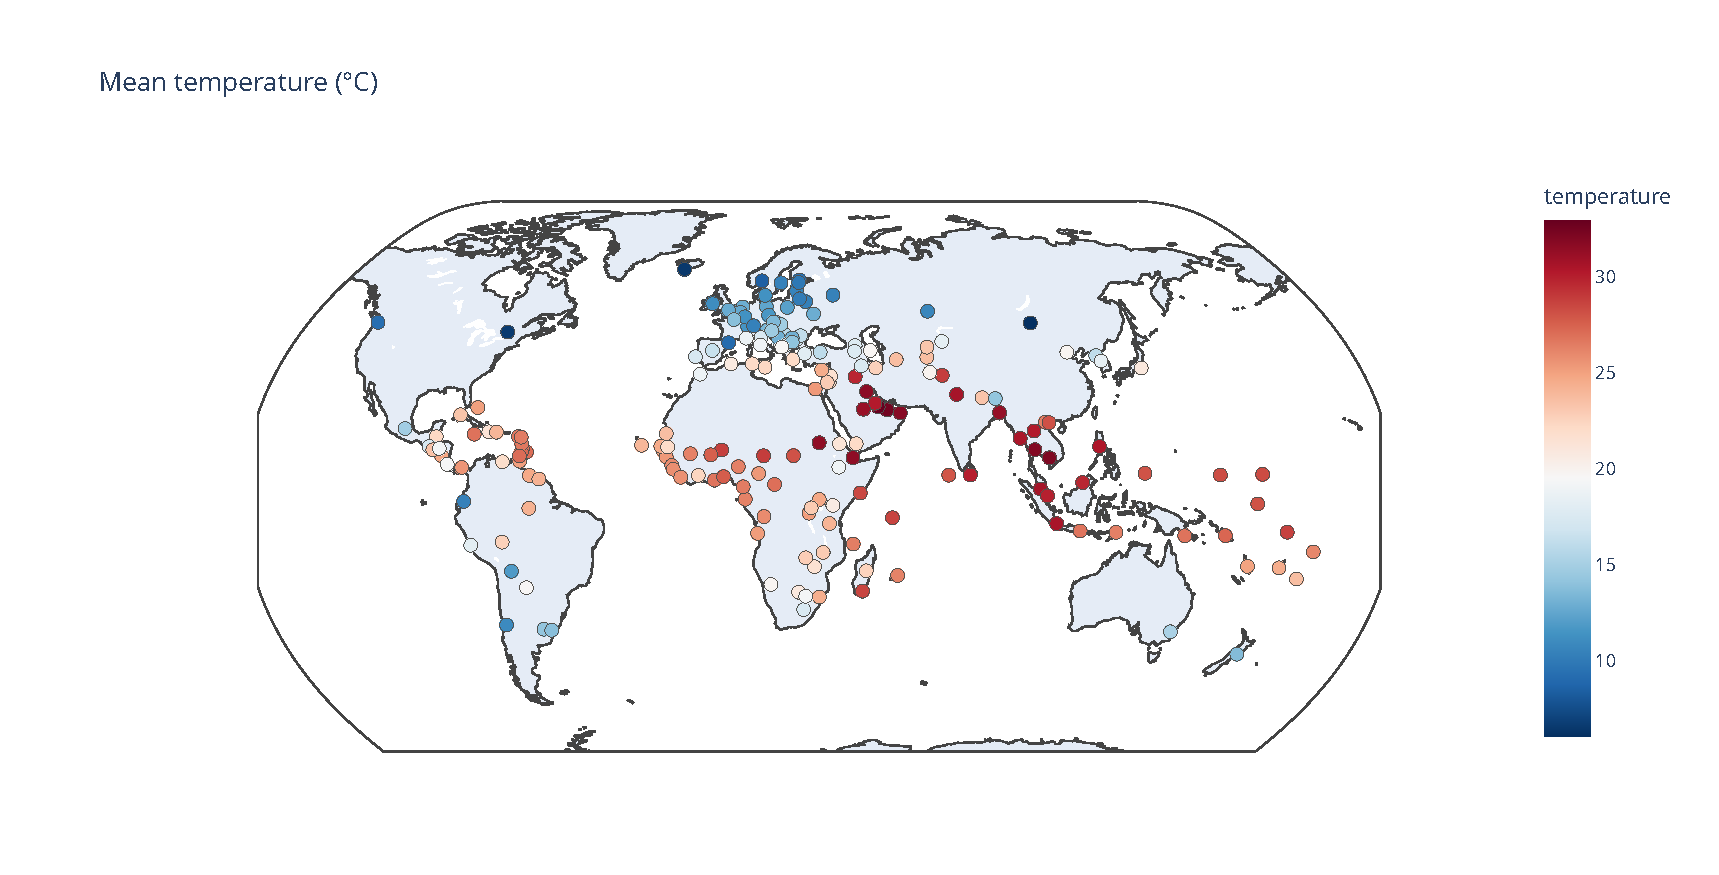
\includegraphics[width=0.85\linewidth]{analyses/geo_map_temperature}
\caption{Mean temperature of the 197 capitals (natural-earth projection).}
\end{figure}
\begin{figure}[H]\centering
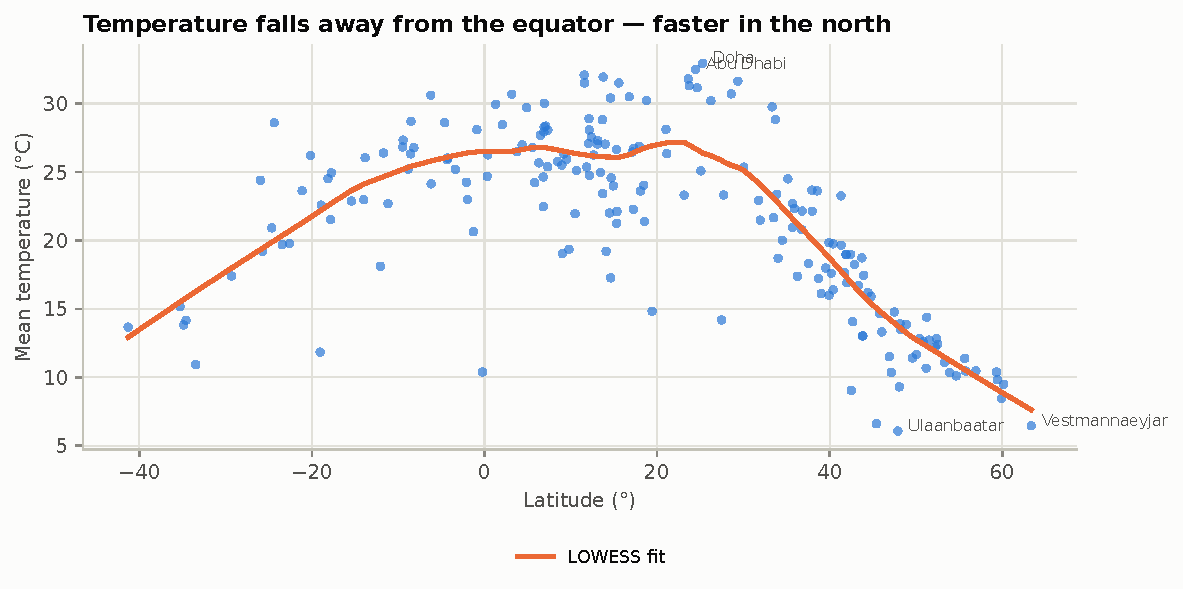
\includegraphics[width=0.85\linewidth]{analyses/spatial_latitude_profile}
\caption{Latitude profile of mean temperature with a LOWESS fit.}\label{fig:latprof}
\end{figure}

\subsection{Geographical patterns}
\tbl{continent_summary.tex}
Doha is the hottest capital in the sample (32.9\,\textdegree C mean) and Ulaanbaatar the coldest
(6.1\,\textdegree C). Asia has both the widest temperature spread and the highest median PM2.5. Europe is
cool and humid with clean air, while Africa and Oceania are warm with narrow ranges
(Figure~\ref{fig:geobox}). Per-country summaries are in \texttt{reports/tables/country\_summary.csv}.

\begin{figure}[H]\centering
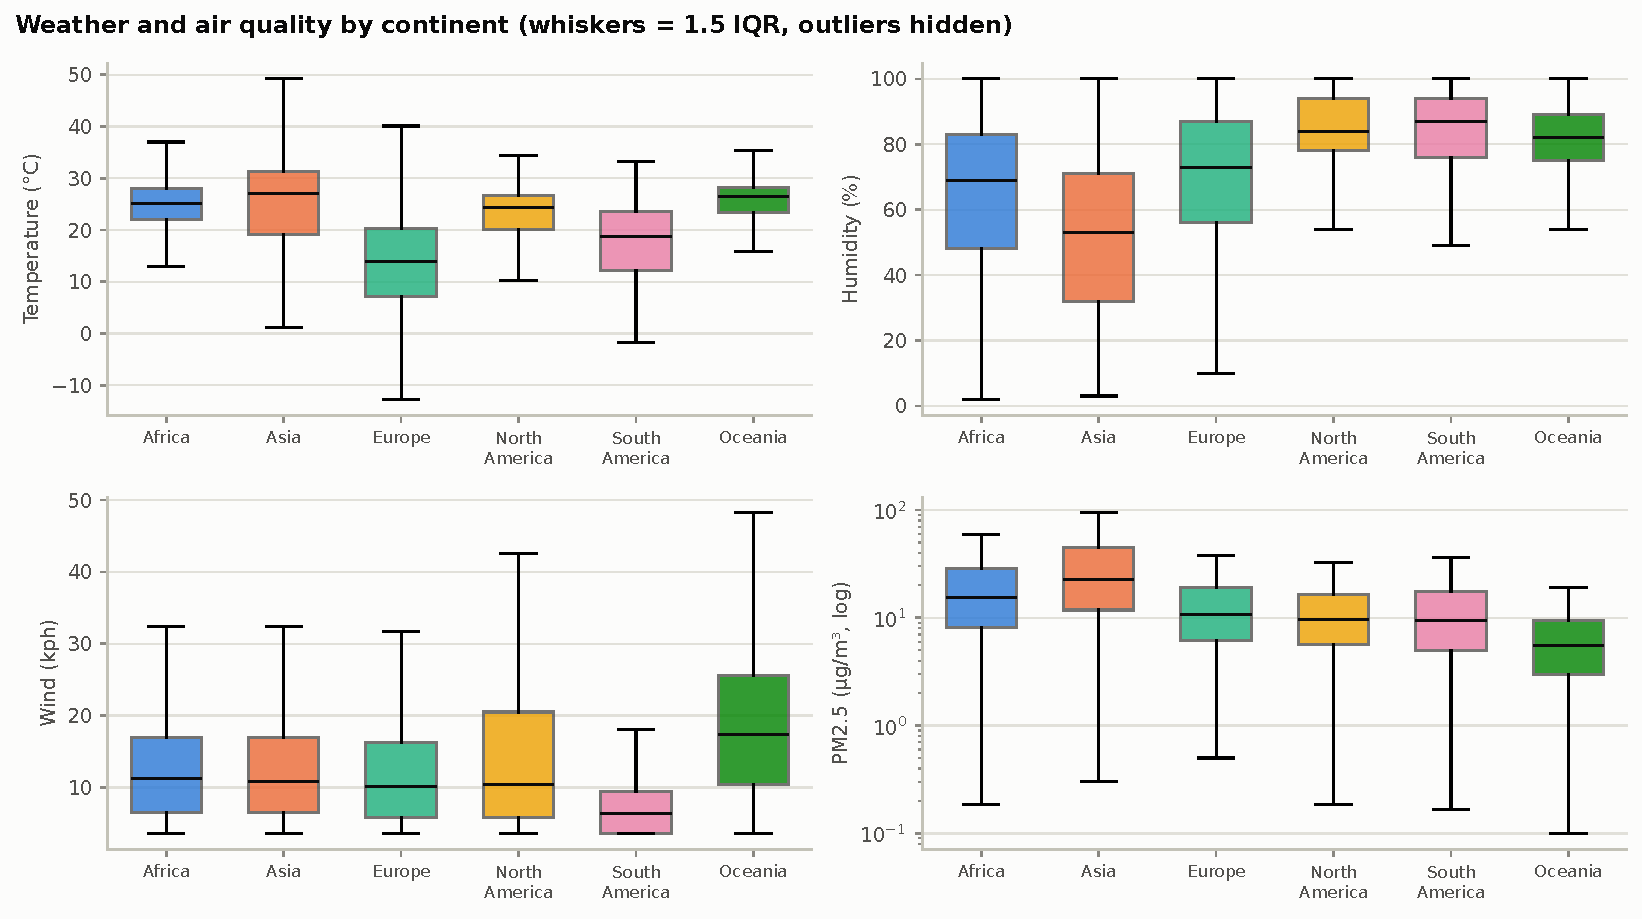
\includegraphics[width=\linewidth]{analyses/geo_continent_boxplots}
\caption{Weather and air quality by continent.}\label{fig:geobox}
\end{figure}
\begin{figure}[H]\centering
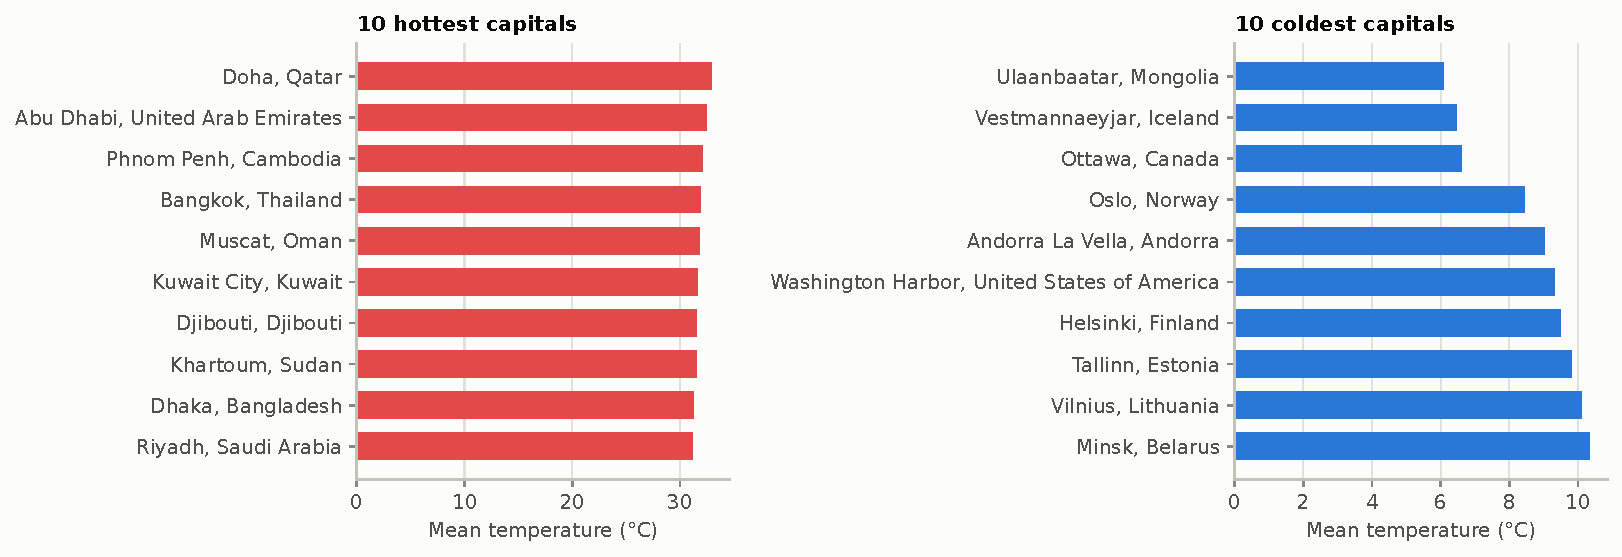
\includegraphics[width=\linewidth]{analyses/geo_hottest_coldest}
\caption{The hottest and coldest capitals by mean temperature.}
\end{figure}
